\documentclass{article}
\usepackage[english]{babel}
\usepackage{amsfonts, amsmath, amssymb, MnSymbol, graphicx, algpseudocode, algorithm, amsthm}
\usepackage{hyperref}

\numberwithin{figure}{section}

%%% Helpers
\newcommand{\algtab}{\hspace{\algorithmicindent}}
\newcommand{\wi}{\omega_i}
\newcommand{\hsigma}{\widehat \Sigma}
\newcommand{\hmu}{\hat \mu}

%%% Shortcuts
\newcommand{\bx}{\mathbf{x}}
\newcommand{\bm}{\mathbf{\mu}}
\newcommand{\bsig}{\mathbf{\Sigma}}
\newcommand{\imgwidth}{.8\textwidth}

%%% Draft helpers (remember to remove when done)
\newcommand{\outline}[2]{\paragraph{\textsc{#1}}\hrulefill~\\{\small\it #2}\\\_\hrulefill}
\newcommand{\todo}[1]{\outline{\large TODO}{#1}}

%%%%%%%%%%%%%%%%%%%%%%%%%%%%%%%%%%%%%%%%%%%%%%%%%%%%%%%%%%%%%%%%%%%%%%%%%%%%%%%%%%%

\title{CAP5638 Project 1\\
\large Classification Using Maximum-likelihood, Parzen Window, and $k$-Nearest Neighbors}
\author{Suhib Sam Kiswani}
\date{October 28, 2015}

%%%%%%%%%%%%%%%%%%%%%%%%%%%%%%%%%%%%%%%%%%%%%%%%%%%%%%%%%%%%%%%%%%%%%%%%%%%%%%%%%%%

\begin{document}
\maketitle

The algorithms were implemented in {\it Python 3.4}, with a dependence on the \textit{scipy} \cite{sp} library. 

The {\bf Speed up using k-d tree} extra credit option was implemented.

%%%%%%%%%%%%%%%%%%%%%%%%%%%%%%%%%%%%%%%%%%%%%%%%%%%%%%%%%%%%%%%%%%%%%%%%%%%%%%%%%%%
\section{Maximum likelihood estimation}
%\subsection{Parametric Forms}
%~~~~~~~~~~~~~~~~~~~~~~~~~~~~~~~~
%\subsubsection{Normal Density}
The discriminant function for the normal density is:

$$g_i(\bx) = \bx^T\mathbf{W}_i\bx + \mathbf{w}_i^T \bx + w_{i0}$$
where:
$$\mathbf{W}_i = -0.5 \bsig_i^{-1}$$
$$\mathbf{w}_i = \bsig_i^{-1} \bm_i$$
$$w_{i0} = -0.5 \bm_i^T \bsig_i^{-1} \bm_i - 0.5\ln \left( \det \bsig_i \right) + \ln P(\omega_i)$$

Using the training samples, the mean and covariance can be estimated with maximum likelihood using the following definitions:
\begin{align*}
\hat\bm_i = \frac{1}{n} \sum^n_{k=1} \bx_k &~& \widehat\bsig_i = \frac{1}{n} \sum^n_{k=1} (\bx_k - \hat\bm_i)(\bx_k - \hat\bm_i)^T
\end{align*}

Which yields:
$$p(\bx|\mathbf{\omega_i}) = \frac{1}{\sqrt{(2 \pi)^n \det \widehat\bsig_i}} \exp\left( -\frac{1}{2} (\bx - \hat\bm_i)^T \widehat\bsig_i^{-1} (\bx - \hat\bm_i) \right)$$

The classification of instance $\bx$ is $\mathbf{\omega_i} = \arg\max_{\mathbf{\omega_i}} \left| p(\bx|\mathbf{\omega_i}) P(\mathbf{\omega_i}) \right|$

%~~~~~~~~~~~~~~~~~~~~~~~~~~~~~~~~
%\subsubsection{Uniform}
%\todo{write out eqns}

%%%%%%%%%%%%%%%%%%%%%%%%%%%%%%%%%%%%%%%%%%%%%%%%%%%%%%%%%%%%%%%%%%%%%%%%%%%%%%%%%%%
\subsection{Experimental Results}
\subsubsection{Iris Data Set}
This method correctly classified $48$ of the $51$ testing samples ($94.1$\% accuracy). The estimated parameters of $\hat\theta$ for each of the classes from the training samples were:
$$\hat\bm_1 = \left( 4.98181818,  3.39090909,  1.45151515,  0.25151515 \right)$$
$$\widehat\bsig_1 = \begin{pmatrix}
    0.10876033 & 0.08619835 & 0.02033058 & 0.01093664\\
    0.08619835 & 0.13597796 & 0.01410468 & 0.00865014\\
    0.02033058 & 0.01410468 & 0.03401286 & 0.00825528\\
    0.01093664 & 0.00865014 & 0.00825528 & 0.0134068
\end{pmatrix}$$

$$\hat\bm_2 = \left( 5.89090909,  2.78787879,  4.26363636,  1.31515152 \right)$$
$$\widehat\bsig_2 = \begin{pmatrix}
    0.2353719  & 0.06867769 & 0.165427   & 0.05256198\\
    0.06867769 & 0.08530762 & 0.07743802 & 0.04442608\\
    0.165427   & 0.07743802 & 0.20110193 & 0.06933884\\
    0.05256198 & 0.04442608 & 0.06933884 & 0.0394674
\end{pmatrix}$$

$$\hat\bm_3 = \left( 6.66060606,  2.94848485,  5.58484848,  1.99393939 \right)$$
$$\widehat\bsig_3 = \begin{pmatrix}
    0.36359963 & 0.11887971 & 0.2851607  & 0.03976125\\
    0.11887971 & 0.10613407 & 0.08861341 & 0.03817264\\
    0.2851607  & 0.08861341 & 0.29219467 & 0.03202938\\
    0.03976125 & 0.03817264 & 0.03202938 & 0.06784206
\end{pmatrix}$$

\subsubsection{UCI Wine Data Set}
This classifier correctly classified 85 out of 89 testing samples ($95.51 \%$ accuracy). The estimated parameters of $\hat\mu_i$ for each of the classes from the training samples were (\emph{note:} the values of sigma are too large to include here):

\begin{align*}
\hat \bm_1 = &~( 13.796, 1.865, 2.446, 16.763, 106.2, 2.885,\\
~& 3.072, 0.289, 2.008, 5.504, 1.07, 3.17, 1108.4 )\\
~&~\\
\hat \bm_2 = &~( 12.281, 1.813, 2.237, 19.803, 93.686, 2.236,\\
~& 2.027, 0.357, 1.585, 3.128, 1.022, 2.745, 532.057 )\\
~&~\\
\hat \bm_3 = &~( 13.172, 2.985, 2.445, 21.375, 99.875, 1.652,\\
~& 0.788, 0.438, 1.184, 7.273, 0.683, 1.658, 616.458 )
\end{align*}



\subsubsection{Handwriting Data set}
This classifier correctly classified 545 out of 2007 testing samples ($27.15 \%$ accuracy). The corresponding values for this data set are too large to include here.

%%%%%%%%%%%%%%%%%%%%%%%%%%%%%%%%%%%%%%%%%%%%%%%%%%%%%%%%%%%%%%%%%%%%%%%%%%%%%%%%%%%
\section{Parzen window estimation}
The window function is:
$$\phi(\bx) = \left\{\begin{matrix}
1 & |\bx_j| \leq 1/2; & j \in [1,...,d]\\
0 & otherwise &
\end{matrix}\right.$$

Where the window width is given by $h_n$ and the volume is given by:
$$V_n = h_n^d$$

\begin{enumerate}
\item {\bf Hypercube Kernel}
$$p(\bx | \omega_i ) = \frac{1}{n} \sum^n_{i=1} \frac{1}{V_n} \phi \left(\frac{\bx - \bx_i}{h_n}\right)$$

\item {\bf Gaussian Kernel}
$$p(\bx | \omega_i ) = \frac{1}{n} \sum^n_{i=1} \frac{1}{V_n} \phi \left(\frac{1}{\sqrt{2\pi}^d V_n} \exp\left[-\frac{1}{2} \left(\frac{\bx - \bx_i}{h_n}\right)^2\right]\right)$$
\end{enumerate}

All data processed by this classifier was transformed using the \emph{z-score}:
$$z_{\omega_i}(\bx) = \frac{\bx - \bm_{\omega_i}}{\mathbf{\sigma_{\omega_i}}}$$

A given point $\bx$ is classified as class $\omega_i$ where: 
$$\mathbf{\omega_i} = \arg\max_{\mathbf{\omega_i}} \left| p(z_{\omega_i}(\bx)|\mathbf{\omega_i}) P(\mathbf{\omega_i}) \right|$$

%%%%%%%%%%%%%%%%%%%%%%%%%%%%%%%%%%%%%%%%%%%%%%%%%%%%%%%%%%%%%%%%%%%%%%%%%%%%%%%%%%%
\subsection{Experimental Results}
For all given data sets, the \emph{Hypercube kernel} was the most accurate method. Overall, this classifier was the slowest (e.g. required the most processing time).

%~~~~~~~~~~~~~~~~~~~~~~~~~~~~~~~~
\subsubsection{Iris Data Set}

\begin{figure}[H]
\centering
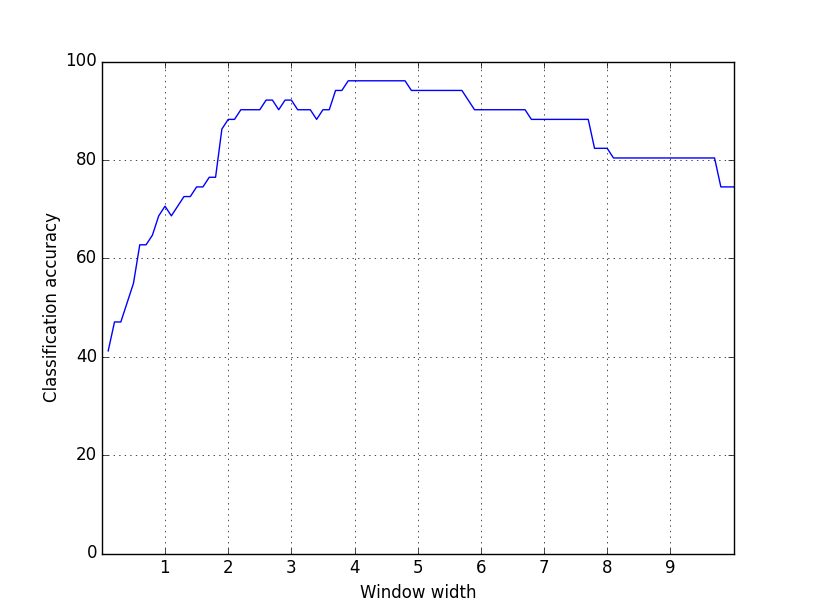
\includegraphics[width=\imgwidth]{p_box_iris}
\caption{Accuracy of the Parzen window classifier using the \emph{Hypercube kernel} across different window widths for the iris data set.}
\label{pb_iris}
\end{figure}

\begin{figure}[H]
\centering
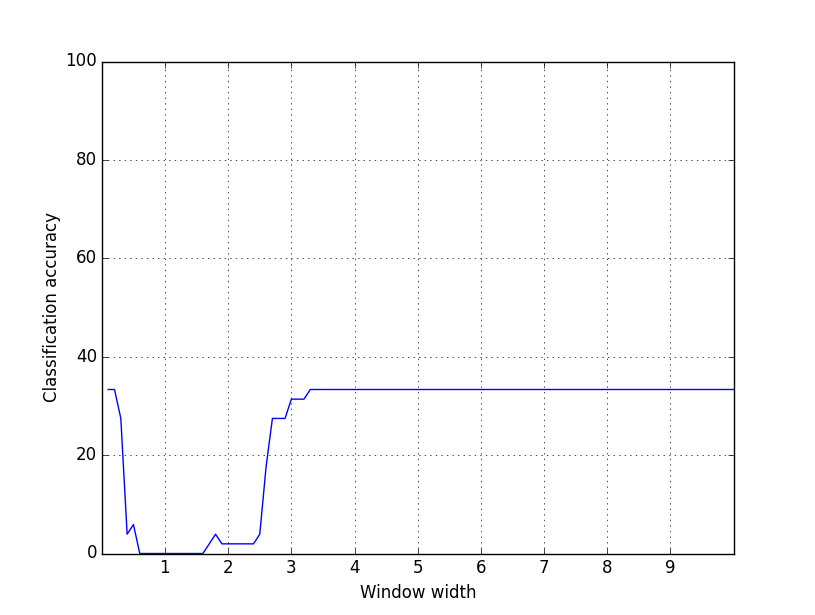
\includegraphics[width=\imgwidth]{pg_iris}
\caption{Accuracy of the Parzen window classifier using the \emph{Gaussian kernel} across different window widths for the iris data set.}
\label{pg_iris}
\end{figure}

%~~~~~~~~~~~~~~~~~~~~~~~~~~~~~~~~
\subsubsection{UCI Wine Data Set}

\begin{figure}[H]
\centering
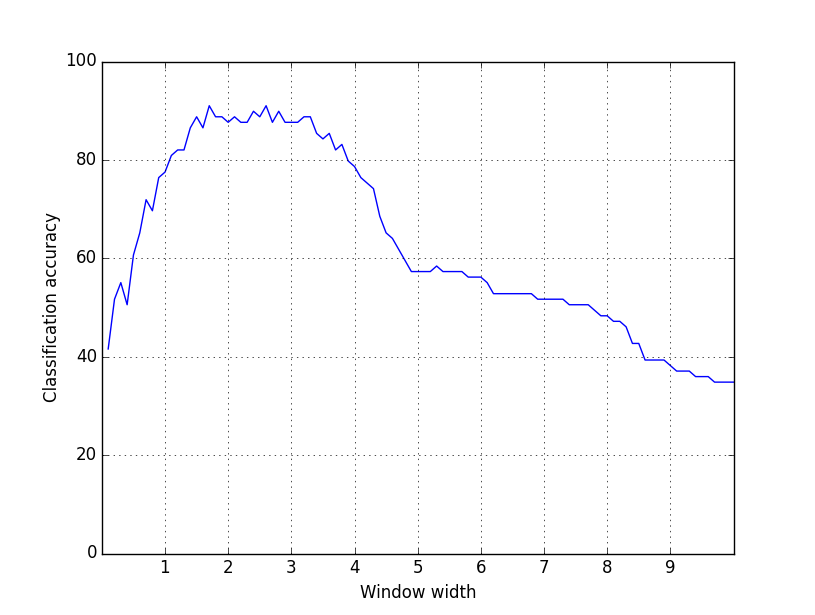
\includegraphics[width=\imgwidth]{p_box_wine}
\caption{Accuracy of the Parzen window classifier using the hypercube window function across different window widths for the wine data set.}
\label{pb_wine}
\end{figure}

\begin{figure}[H]
\centering
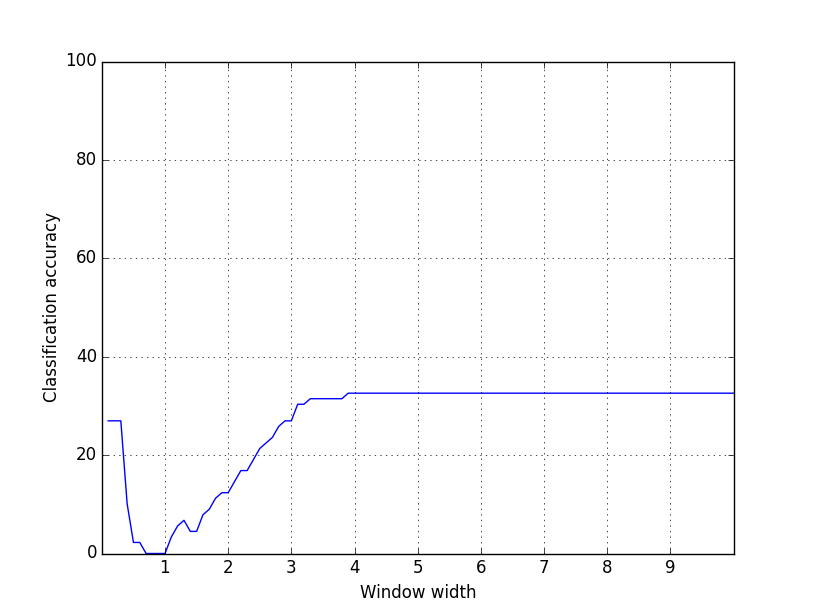
\includegraphics[width=\imgwidth]{pg_wine}
\caption{Accuracy of the Parzen window classifier using the \emph{Gaussian kernel} across different window widths for the wine data set.}
\label{pg_wine}
\end{figure}


%~~~~~~~~~~~~~~~~~~~~~~~~~~~~~~~~
\subsubsection{Handwritten Digits Data Set}
The Parzen window classifier failed to perform very well for this data set, in addition to its extremely slow run-time (which is expected, given the high dimensionality of this data set).

\begin{figure}[H]
\centering
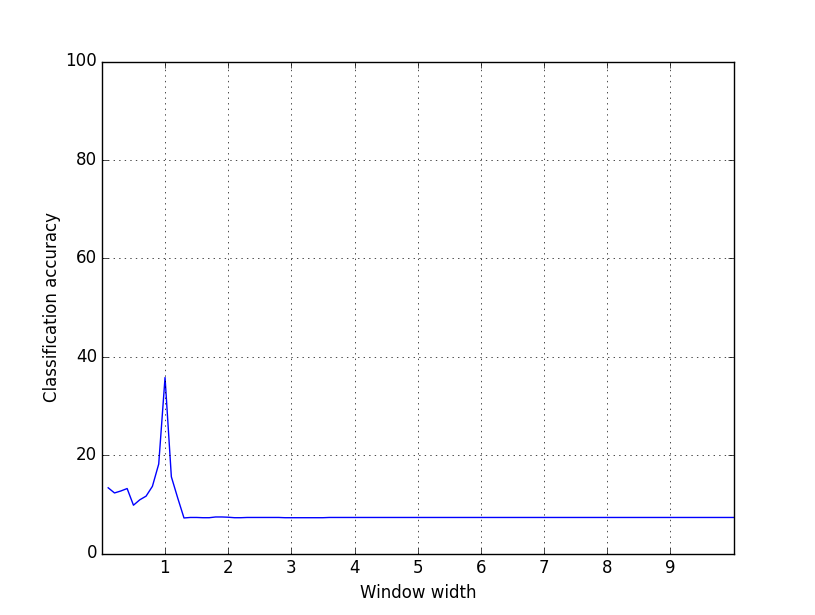
\includegraphics[width=\imgwidth]{pb_hand}
\caption{Accuracy of the Parzen window classifier using the \emph{Hypercube kernel} across different window widths for the handwriting data set.}
\label{pb_hand}
\end{figure}

\begin{figure}[H]
\centering
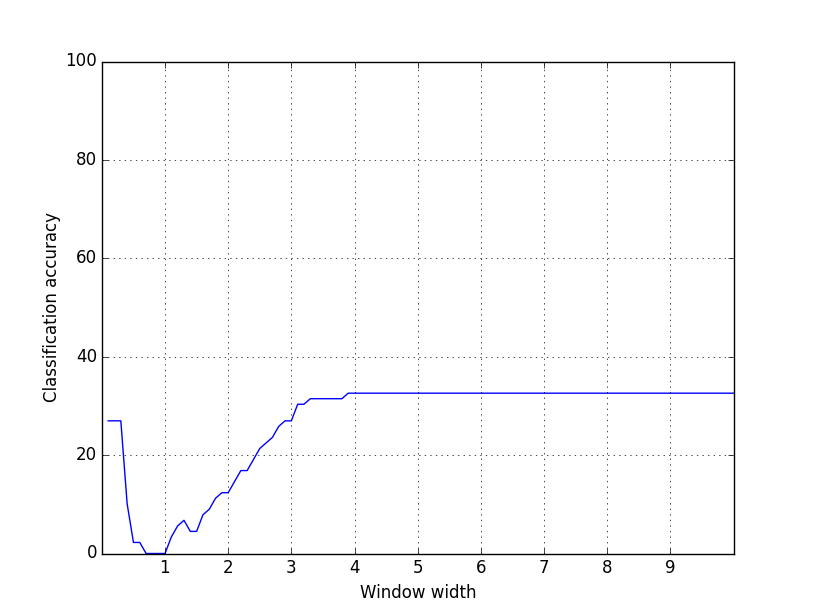
\includegraphics[width=\imgwidth]{pg_wine}
\caption{Accuracy of the Parzen window classifier using the \emph{Gaussian kernel} across different window widths for the handwriting data set.}
\label{pg_hand}
\end{figure}

%%%%%%%%%%%%%%%%%%%%%%%%%%%%%%%%%%%%%%%%%%%%%%%%%%%%%%%%%%%%%%%%%%%%%%%%%%%%%%%%%%%
\section{$k$-nearest neighbors}
The $k$-nearest neighbors classifier was implemented using a $kd$-tree, subdividing along the median of the training data. This distance metric $d$ used for this classifier was Euclidean distance ($||\bx - \textbf{y}||$).

%%%%%%%%%%%%%%%%%%%%%%%%%%%%%%%%%%%%%%%%%%%%%%%%%%%%%%%%%%%%%%%%%%%%%%%%%%%%%%%%%%%
\subsection{Experimental Results}

%~~~~~~~~~~~~~~~~~~~~~~~~~~~~~~~~
\subsubsection{Iris Data Set}
\begin{figure}[H]
\centering
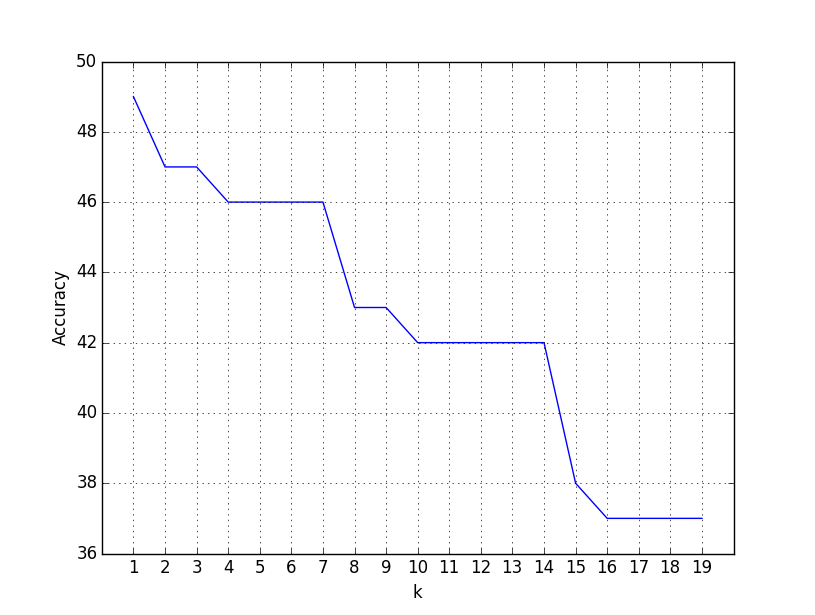
\includegraphics[width=\imgwidth]{knn_kd_iris}
\caption{The number of correct classifications by$k$-nearest neighbors classifier using a $kd$-tree for $1 \leq k \leq 19$ on the iris data set.}
\label{knn:kd:iris}
\end{figure}

The $k$-nearest neighbors classifier achieved a maximum classification rate of $96.08\%$ accuracy for $k=1$. Performance of this classifier degraded rapidly, which is most likely a side of effect of the fact that \emph{sepal width} had poor class correlation, yet was given equal weight as other  features. This can be improved by using applying a normalizing transform to the data set, or choosing a better suited distance metric for this data set.

%~~~~~~~~~~~~~~~~~~~~~~~~~~~~~~~~
\subsubsection{UCI Wine Data Set}
\begin{figure}[H]
\centering
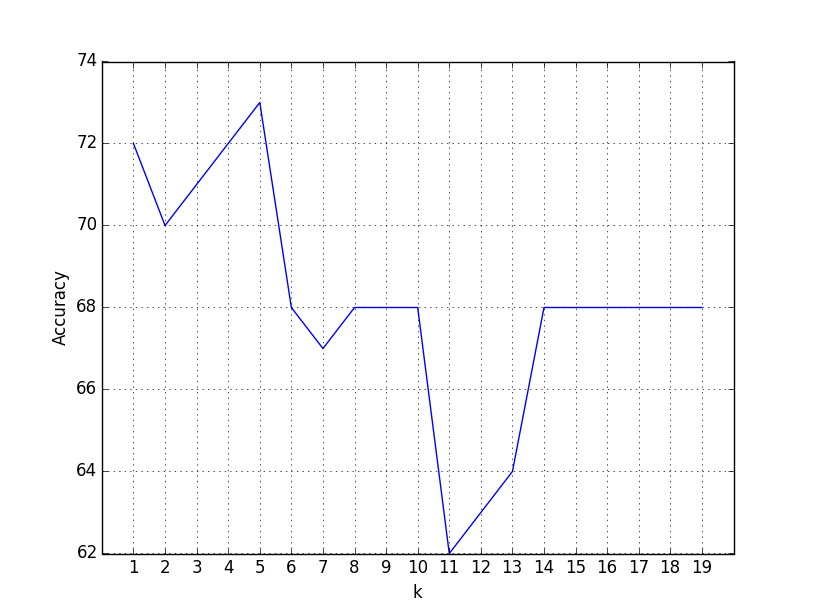
\includegraphics[width=\imgwidth]{knn_kd_wine}
\caption{The number of correct classifications by$k$-nearest neighbors classifier using a $kd$-tree for $1 \leq k \leq 19$ on the wine data set.}
\label{knn:kd:wine}
\end{figure}

Here, the $k$-nearest neighbors classifier achieved a maximum classification rate of $82.02\%$ accuracy for $k=5$. Notably, in this instance, the classifier could not exceed the threshold of $90\%$ accuracy. Most likely this is due to the fact that Euclidean distance may not be a suitable distance metric for this data set. In the \emph{README} included with this data set, a $1$-NN classifier achieved $96.1\%$ accuracy on z-transformed data. As such, that may result in a significant improvement (as was the case in the iris data set). 

%~~~~~~~~~~~~~~~~~~~~~~~~~~~~~~~~
\subsubsection{Handwritten Digits Data Set}
\begin{figure}[H]
\centering
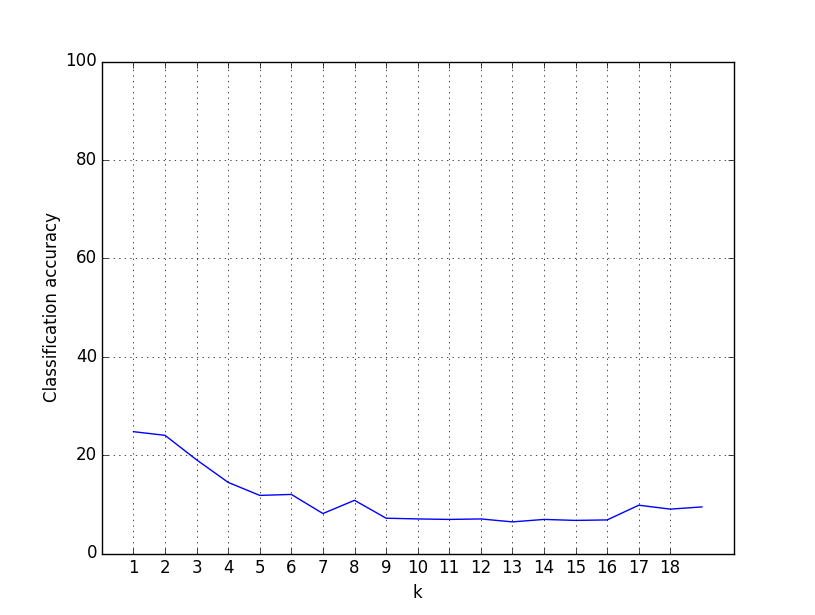
\includegraphics[width=\imgwidth]{knn_kd_hands}
\caption{The accuracy of the $k$-nearest neighbors classifier using a $kd$-tree for $1 \leq k \leq 19$ on the handwriting data set.}
\label{knn:kd:hands}
\end{figure}

Again, the optimal $k$ for the classifier is $1$, with 497 correct classifications out of 2007 ($24.76\%$ accuracy). No transformations were applied to this data set, as reflected in the poor accuracy of this classifier.

%%%%%%%%%%%%%%%%%%%%%%%%%%%%%%%%%%%%%%%%%%%%%%%%%%%%%%%%%%%%%%%%%%%%%%%%%%%%%%%%%%%
\section{Analysis}

\begin{enumerate}
\item {\bf Iris data set.}
All methods performed very well on the iris data set. This is most likely due to the fact that there is a high class correlation for two of the features.

\item {\bf Wine data set.}
This data set proved more difficult for my implementation of the classifiers.

\item {\bf Handwriting data set.}
Every classifier seemed to have difficulties properly classifying samples from this data set. Most likely, this is because the domain of each feature was $[-1, -1]$ and no normalizing transformations were used in any of the classifiers. This is in addition to the difficulties in classifying high-dimensional data.
\end{enumerate}

Also, there is most likely an error in the implementation of the Gaussian kernel for the Parzen Windows classifier, since it performed atrociously on every data set.





%%%%%%%%%%%%%%%%%%%%%%%%%%%%%%%%%%%%%%%%%%%%%%%%%%%%%%%%%%%%%%%%%%%%%%%%%%%%%%%%%%%

\begin{thebibliography}{9}

\bibitem{sp}
    Jones E, Oliphant E, Peterson P, \emph{et al.}
    {\bf SciPy: Open Source Scientific Tools for Python}, 2001-,
    \url{http://www.scipy.org/} [Online; accessed 2015-10-24].

\end{thebibliography}

%%%%%%%%%%%%%%%%%%%%%%%%%%%%%%%%%%%%%%%%%%%%%%%%%%%%%%%%%%%%%%%%%%%%%%%%%%%%%%%%%%%

\end{document}